\section{Results}
\label{sec:results}

Numerical solutions for the considered initial-boundary value problems were computed with a finite 
difference method in space and \textcolor{red}{temporal discretization}. 
For the wave equation, the Lax--Wendroff scheme \cite{LW60,LeV92} was utilized. These solutions were 
used to train the data-driven neural network. 

We have investigated several aspects of the numerical simulations. First, the convergence of the 
optimization process was studied, where we explored which terms of the multi-objective 
loss functional were easily or hard to minimize. Then, of course, the quality of the solution 
predicted by the networks was studied. On the one hand, we considered exactly the interval were the 
data came from. And on the other hand, we exploreed what happens if a somewhat larger time 
interval is considered, i.e., the predictions of the network were applied to an unseen situation. 
We studied also the impact of using different activation functions. For the sake of brevity, only 
selected and representative results will be presented. 


\subsection{Wave equation}
\label{subsec:wave_res}

We consider equation \eqref{eq:wave} for $x \in [0,1]$, $t \in [0,1]$, and $c =1$.  A solution of this 
equation is given by 
\[
u(x,t) = \frac{1}{2} \sin (\pi x) \cos(\pi t) + \frac{1}{3} \sin (3\pi x) \sin (3 \pi t).  
\]
This function is for the boundary conditions a $u(0,t) = u(1,t) =  0$ and the initial 
conditions 
\[
u_0  = u(x,0)  = \frac{1}{2} \sin (\pi x), \quad \frac{\partial u}{\partial t}(x,0) = \pi  \sin (3 \pi x)
\]
the solution of the initial-boundary value problem \eqref{eq:wave} -- \eqref{eq:wave_cond}.


The finite difference solution was obtained with $\Delta t = \Delta x = 0.0025$, i.e., with $400$ 
discrete steps both in time and space. The training of the data-driven network was performed only 
in the time interval $[0,0.8]$. The numerical solution at every timestep was used. Likewise, 
the PINNs was also trained for $t \in (0,0.8)$. The application of the trained networks to an 
unseen situation consists in predicting the solution in $[0.8,1]$. 

\begin{figure}[t!]
\begin{center}
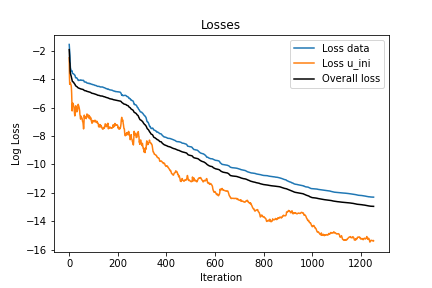
\includegraphics[width=0.45\linewidth]{../Code/B1/losses/combined_losses_reduction_data.png}
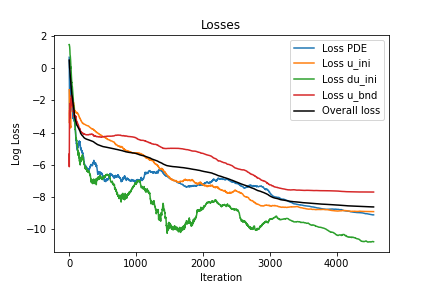
\includegraphics[width=0.45\linewidth]{../Code/B1/losses//combined_losses_reduction_PINNs.png}
\end{center}
\caption{Wave equation. Activation function $\tanh(x)$. Convergence of the optimization process 
for minimizing the loss functionals and their individual terms. Note the different scaling of the 
abscissa.}\label{fig:wave_loss_contributions}
\end{figure}

First, results for the activation function $\tanh(x)$ will be presented and discussed. 
As already explained in Section~\ref{sec:neuralnets}, the formulation of the loss functional is 
different for both networks. Figure~\ref{fig:wave_loss_contributions} illustrates how the each of the 
residual term in \eqref{eq:loss} is minimized in the multi-objective optimization. Moreover, we see 
that the estimation of hyperparameters requires less iterations using 
the data-driven network. However, the performance for the PINN is quite also satisfactory given 
no pre-computed solutions are required to train the network.   
\textcolor{red}{the pictures need more explanations. I do not understand that the overall loss 
is smaller than the largest individual loss.}

\begin{figure}[t!]
\begin{center}
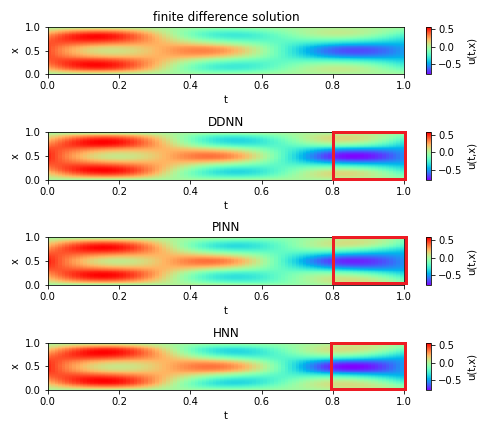
\includegraphics[width=0.4\linewidth]{../Code/B1/plots/colormap.png}
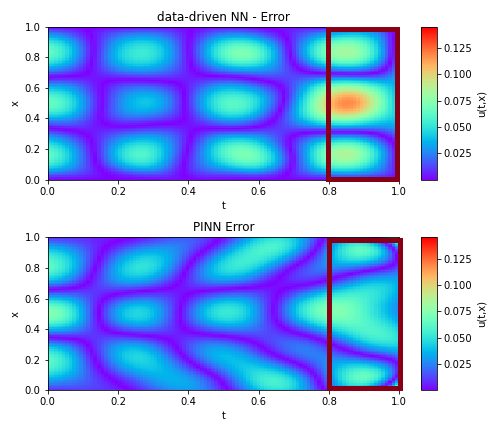
\includegraphics[width=0.4\linewidth]{../Code/B1/plots/error_colormap.png}
\end{center}
\caption{Wave equation. Activation function $\tanh(x)$. Left: Comparison of solution $u(x,t)$ obtained from data and physics trained network against reference solution. Right: The error map plotted for solutions obtained from data and physics trained network.\\
\textcolor{red}{headlines of the pictures: 'finite difference solution', 'data-driven NN', 'PINN'}\\
\textcolor{red}{on right: data-driven picture above PINN picture (same sequence as on left)}\\
\textcolor{red}{'400' is irritating, since training for data used only 320 (321) finite difference solutions}
}\label{fig:wave_sol_error}
\end{figure}

Figure~\ref{fig:wave_sol_error} (left) shows the comparison of the results of the 
data- and physics-driven neural networks to the finite difference solution. 
In the right-hand side pictures the error maps for both networks are depicted, where the 
(abolute value of the) error in each node in space and time was computed. 
Whereas the errors in $t\in[0,0.8]$ are of the same size for both networks, at most of the order $0.075$,
it can be seen that the PINNs performed better than the data-trained network for $t\in[0.8,1]$.
\textcolor{red}{Before, the sentence was the other direction. I changed in it accordance with the labels 
of the pictures.}

\begin{figure}[t!]
\begin{center}
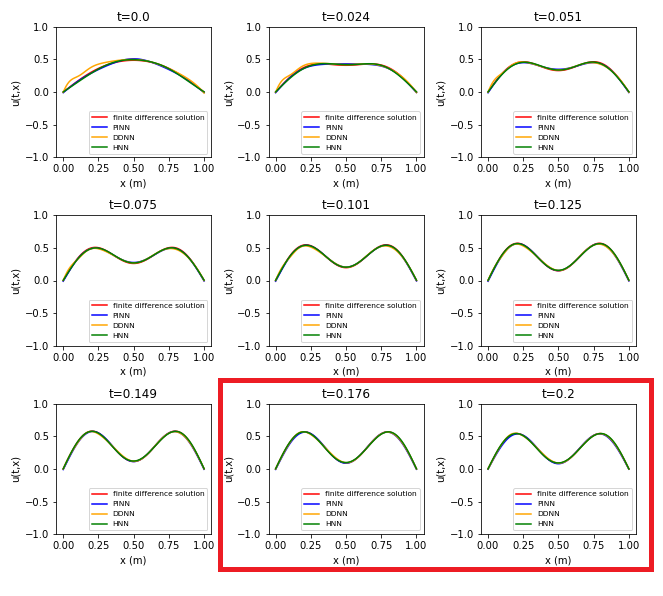
\includegraphics[width=0.45\linewidth]{../Code/B1/plots/wave_numerics.png}
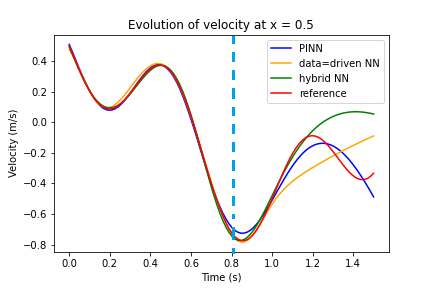
\includegraphics[width=0.45\linewidth]{../Code/B1/plots/evolution_plot.png}
\end{center}
\caption{Wave equation. Activation function $\tanh(x)$. Comparison of the finite difference
solution against solutions obtained from the data- and physics-trained networks. 
Left: $u(x,t)$ plotted at some time instances $t$. Right: Temporal evolution of the error
at $x=0.5$.\\
\textcolor{red}{once more, '100' and '400' are disturbing, it should be '81' and '321'.}\\
\textcolor{red}{the same things should have in both pictures the same colors.}\\
\textcolor{red}{For $t\approx 0.85$, the yellow and green curce should be much more away from 
the red curve in the right picture, because the error is large.}}
\label{fig:wave_evolution}
\end{figure}

Figure~\ref{fig:wave_evolution} presents more information on the prediction of the wave velocity. 
In addition to using all time steps in $[0,0.8]$ for learning the data-driven network, also the 
case of using only every $4$th time step. One can observe that in $[0,0.8]$ the predictions 
from all networks are quite similar. However, there are differences for the unseen situation.
The data-driven network lead to predictions with a much larger error in the middle of the interval for $t=0.879$. And for longer time horizons, $t>1.2$, the PINN prediction is significantly more reliable.
\textcolor{red}{To be honest, I do not see the new information of the left picture.}


\subsection{Shallow water equation}

The initial boundary value problem \eqref{eq:swe} -- \eqref{eq:swe_ic_bc} for the shallow water 
equations was solved in $(x,t) \in [0,1]\times [0,0.2]$. The velocity is considered to be at equilibrium at $t=0$, i.e. $u(x, 0) = 0$.
Two different initial profiles for 
$h(x,0)$ will be considered, leading to solutions with different features.
\textcolor{red}{provide 
information about compuation of the solution to compare with: discretizations in time and space, 
finenss}

Besides the data-driven neural network and the PINN, we will study for this example also a hybrid network, where the loss functional is the following linear combination of the data part \eqref{eq:fct_data} and the physics part \eqref{eq:fct_phys} \textcolor{red}{give concrete linear combination}
All networks will be trained with the numerical solution from $[0,0.15]$ and the unsee situation 
is the solution in $(0.15,0.2]$. 


  
\subsubsection{Initial profile $h(x, 0)$ leading to a smooth solution}

\begin{figure}[t!]
\begin{center}
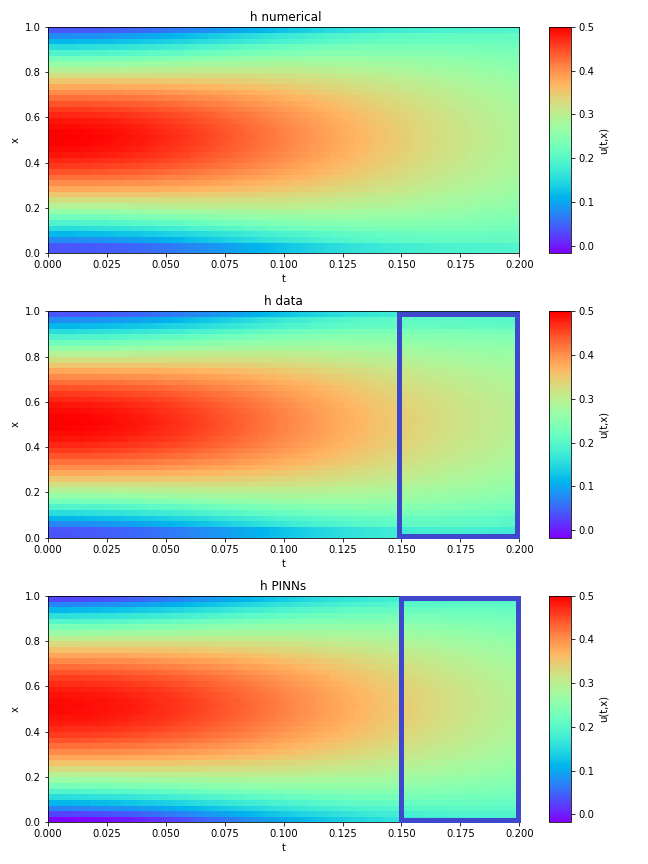
\includegraphics[width=0.45\linewidth]{./plots/h_colormap_b1.png}
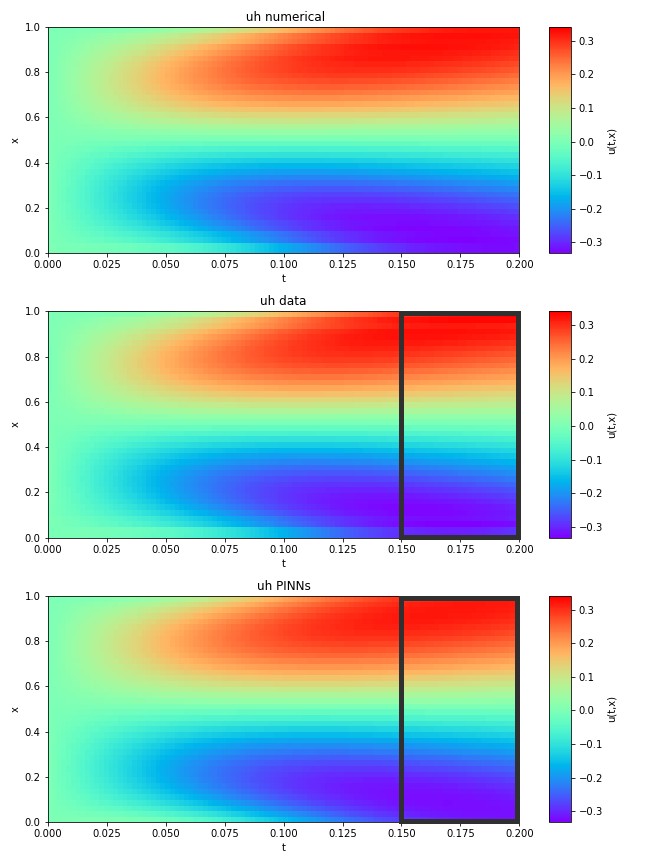
\includegraphics[width=0.45\linewidth]{./plots/uh_colormap_b1.png}
\end{center}
\caption{Shallow water equations, smooth solution. ctivation function $\tanh(x)$. Solution of 
the initial boundary value problem (top), solution obtained with the data-driven neural network (middle), 
solution obtained with the PINN (bottom).}
\label{fig:b1_swe_sol}
\end{figure}

The initial profile of the height considered in this example has the form  $h(x,0) =\frac{1}{2} \sin (\pi x)$.
The numerical solution of  \eqref{eq:swe} -- \eqref{eq:swe_ic_bc} can be seen in the upper part of 
Figure~\ref{fig:b1_swe_errors}.

\begin{figure}[t!]
\begin{center}
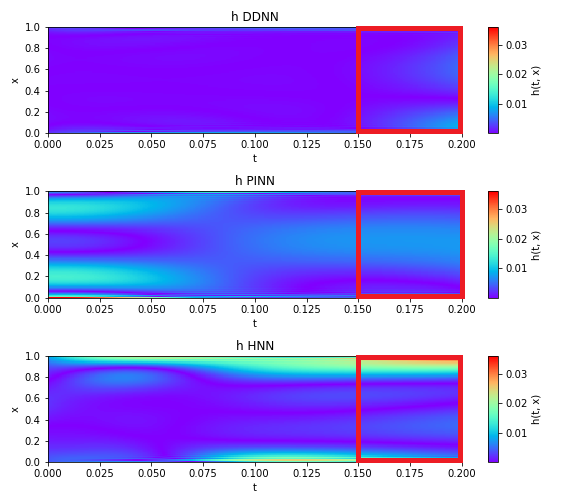
\includegraphics[width=0.45\linewidth]{../Code/B2/plots/h_errorplot_b1.png}
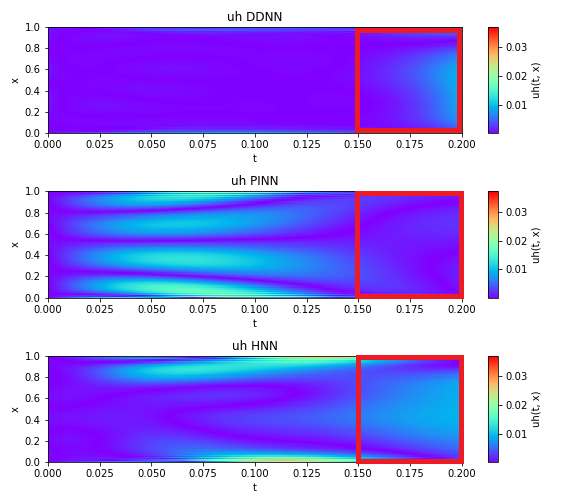
\includegraphics[width=0.45\linewidth]{../Code/B2/plots/uh_errorplot_b1.png}
\end{center}
\caption{
Error maps of $h(x, t)$ and $u(x,t)$ for the data driven neural network (left) and the PINN (right).}\label{fig:b1_swe_errors}
\end{figure}

Comparisons of the results obtained with the data-driven neural network and the PINN are presented
in this picture as well and the corresponding errors in Figure~\ref{fig:b1_swe_errors}. For the 
seen interval $[0,0.15]$, the results with the data driven neural network are clearly 
more accurate. This situation changes somewhat for the unseen interval, where the velocity error
for the data driven network becomes large at the left spatial boundary and $t\to 0.2$. But altogether, 
one can conclude that both neural networks give satisfactory results for $t\in[0,0.2]$


\begin{figure}[t!]
\begin{center}
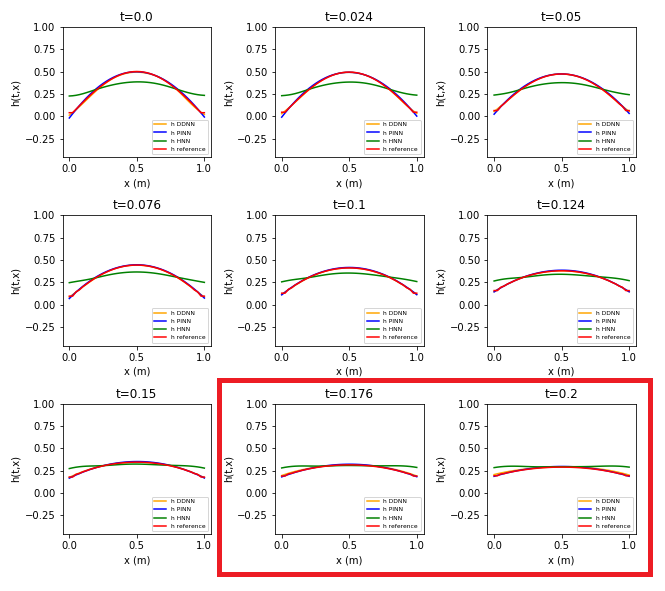
\includegraphics[width=0.45\linewidth]{../Code/B2/plots/h_b1.png}
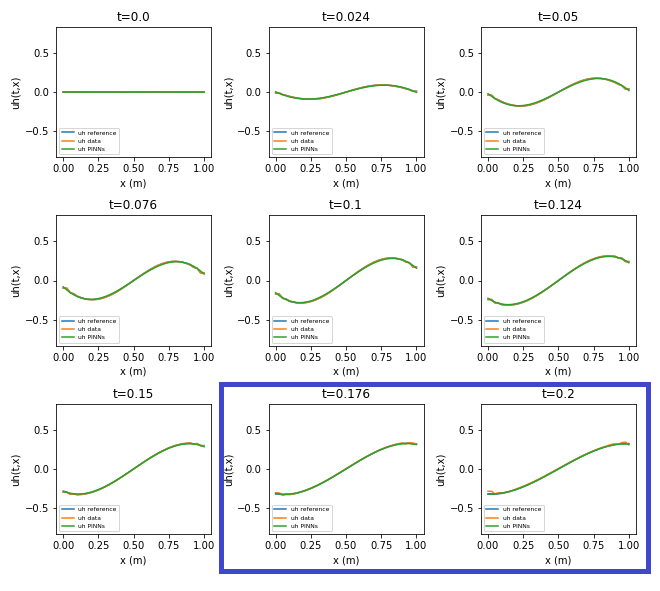
\includegraphics[width=0.45\linewidth]{../Code/B2/plots/uh_b1.png}
\end{center}
\caption{Shallow water equations, smooth solution. ctivation function $\tanh(x)$.  Solutions $h(x, t)$ and $u(x,t)$ plotted at different $t$.
\textcolor{red}{Do we need this picture? What are the new information?}}\label{fig:b1_swe_time}
\end{figure}


\begin{figure}[t!]
\begin{center}
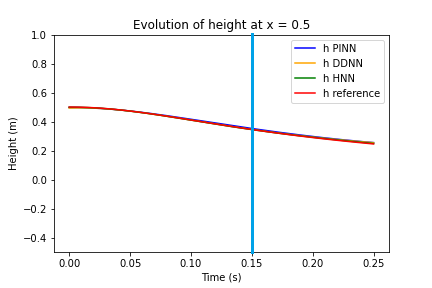
\includegraphics[width=0.45\linewidth]{../Code/B2/plots//h_evolution_plot_b1}
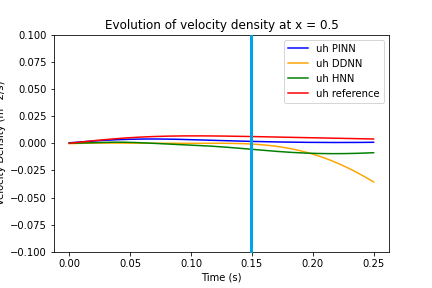
\includegraphics[width=0.45\linewidth]{../Code/B2/plots/uh_evolution_plot_b1}
\end{center}
\caption{Shallow water equations, smooth solution. ctivation function $\tanh(x)$.  Solutions $h(x=0.5,t)$ and $u(x=0.5, t)$ forward-in-time predictions.}\label{fig:b1_swe_time_x05}
\end{figure}

However, extending the unseen time interval a little bit further, the prediction from the 
data-driven neural network becomes unreliable, compare Figure~\ref{fig:b1_swe_time_x05}.

\textcolor{red}{shall we present results for the hybrid network here, or just say that they are not 
much different, because the results for the other networks are not much different as well?}

\subsubsection{Initial profile $h(x,0)$ leading to a solution with shocks}

We solved the shallow water equation for a slightly more realistic dam flow example where the initial profile of $h(x,0) =2+sin (2\pi x) $ results in a more complex wave propogation. The velocity is considered to be at equilibrium at $t=0$, i.e. $u(x, 0) = 0$. 
\par
\noindent
The solutions are compared against the reference/numerical solutions in figure \ref{fig:b2_swe_sol}. Both data and physics driven network learn the solution within a $10^{-2}$ accuracy as can be seen in figure \ref{fig:b2_swe_errors}.
\par
\noindent
For feed forward predictions of the solution for the time that's not incorporated in the training, the hybrid approach works better than PINNs. It can be seen in figure \ref{fig:b2_swe_time} that when looked on a micro scale, data-driven network overestimates the predicted velocities. Overall, learning for both networks is quite satisfactory for the case of gradual propogation of the wave. 

\begin{figure}[t!]
\begin{center}
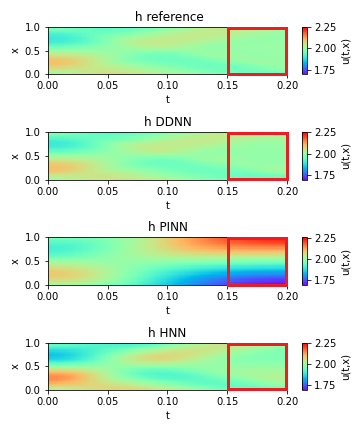
\includegraphics[width=0.45\linewidth]{../Code/B3/plots/h_colormap_b2.png}
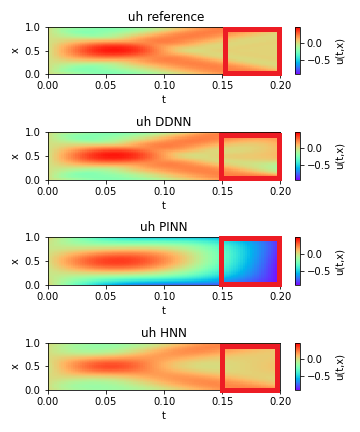
\includegraphics[width=0.45\linewidth]{../Code/B3/plots/uh_colormap_b2.png}
\end{center}
\caption{Case 2.2  Comparison of the $h(x,t)$ $and u(x,t)$ obtained from numerical, data and model-trained network}\label{fig:b2_swe_sol}
\end{figure}




\begin{figure}[h!]
\begin{center}
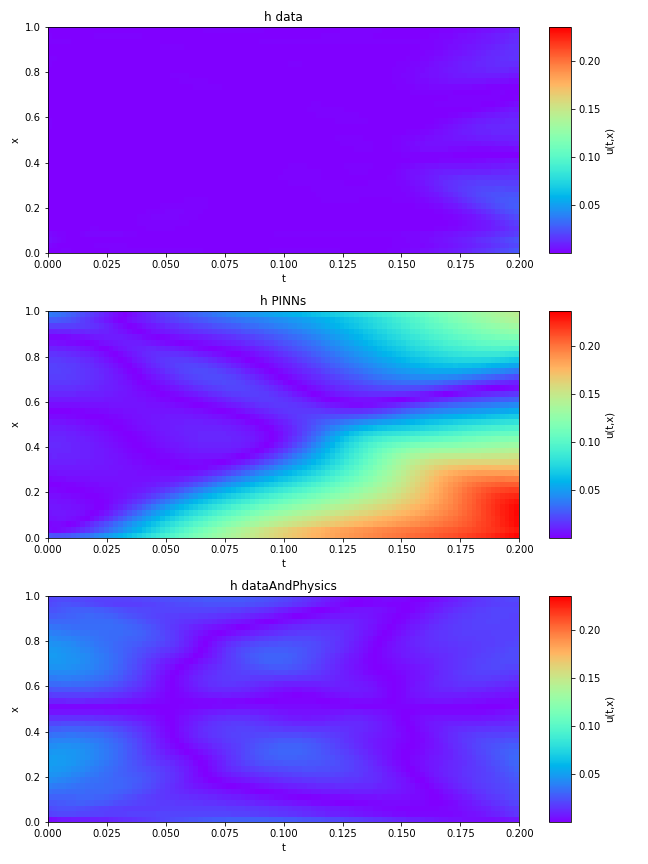
\includegraphics[width=0.45\linewidth]{../Code/B3/plots/h_errorplot_b2.png}
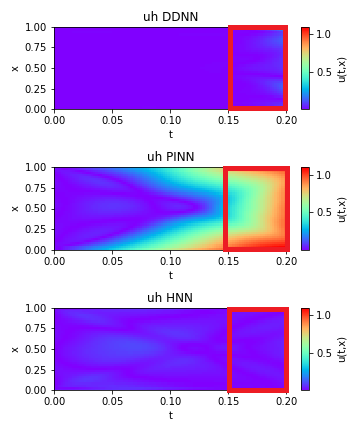
\includegraphics[width=0.45\linewidth]{../Code/B3/plots/uh_errorplot_b2.png}
\end{center}
\caption{Case 2.2: The error maps of $h(x, t)$ and $u(x,t)$ is plotted as a color map.}\label{fig:b2_swe_errors}
\end{figure}

\begin{figure}[h!]
\begin{center}
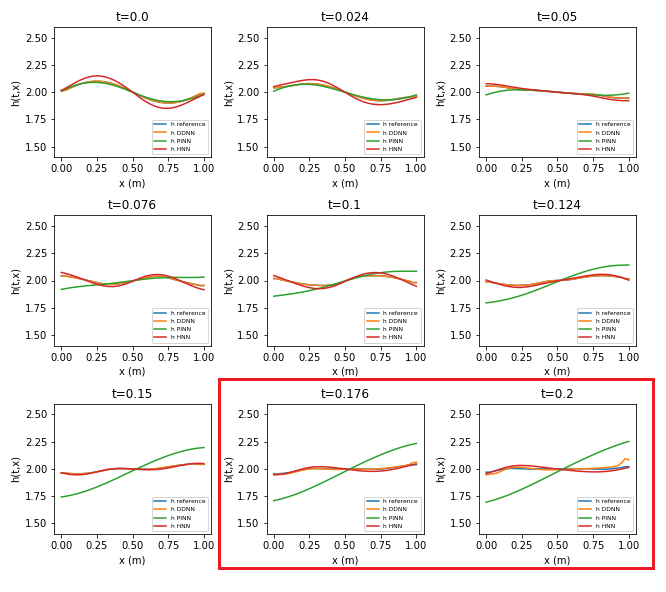
\includegraphics[width=0.45\linewidth]{../Code/B3/plots/h_b2.png}
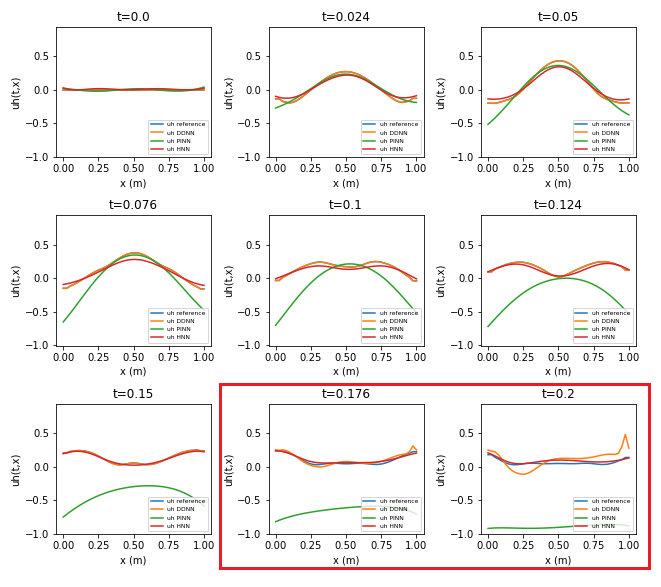
\includegraphics[width=0.45\linewidth]{../Code/B3/plots/uh_b2.png}
\end{center}
\caption{Case 2.2: Solutions $h(x, t)$ and $u(x,t)$ plotted at different $t$.}\label{fig:b2_swe_time}
\end{figure}


\begin{figure}[h!]
\begin{center}
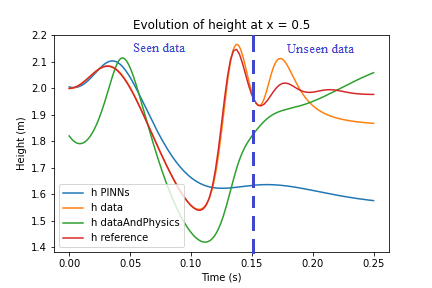
\includegraphics[width=0.45\linewidth]{./plots/h_evolution_plot_b2.png}
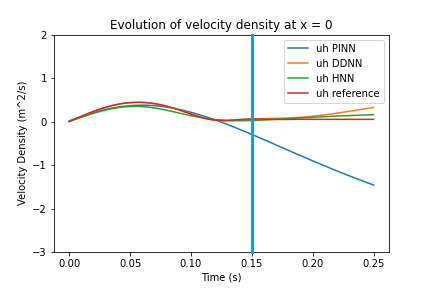
\includegraphics[width=0.45\linewidth]{../Code/B3/plots/uh_evolution_plot_b2.png}
\end{center}
\caption{Case 2.2: Solutions $h(x=0.5,t)$ and $u(x=0.5, t)$ forward-in-time predictions.}\label{fig:b2_swe_time_x05}
\end{figure}
